\documentclass[a4paper,oneside,10pt]{article}
\usepackage[utf8]{inputenc}
\usepackage[T1]{fontenc}

\usepackage{makeidx}
\usepackage{graphicx}
\usepackage[french]{babel}
\usepackage{amsmath}
\usepackage{amssymb}
\usepackage{mathrsfs}
\usepackage{lmodern}
\usepackage{listings}
\usepackage{caption}
\usepackage{pgfplots}
\usepackage{hyperref}
\usepackage{url}
\usepackage{csquotes}
\usepackage{mathabx}
\usepackage{fancyhdr}
\pagestyle{fancy}
\fancyhead[L]{\thepage}
\fancyhead[R]{Ensemble Dominant Connexe Glouton}
\cfoot{}

\usepackage{afterpage}
\newcommand\blankpage{%
    \null
    \thispagestyle{empty}%
    \addtocounter{page}{-1}%
    \newpage
}

\pgfplotsset{compat=1.14}

\usepackage{listings}
\usepackage{color}

\definecolor{dkgreen}{rgb}{0,0.6,0}
\definecolor{gray}{rgb}{0.5,0.5,0.5}
\definecolor{mauve}{rgb}{0.58,0,0.82}

\lstset{frame=tb,
  language=Java,
  aboveskip=3mm,
  belowskip=3mm,
  showstringspaces=false,
  columns=flexible,
  basicstyle={\small\ttfamily},
  numbers=none,
  numberstyle=\tiny\color{gray},
  keywordstyle=\color{blue},
  commentstyle=\color{dkgreen},
  stringstyle=\color{mauve},
  breaklines=true,
  breakatwhitespace=true,
  tabsize=3
}

\newtheorem{lemma}{Lemma}

\makeindex
\begin{document}
\title{Algorithme Li et al. : ensemble dominant connexe glouton}
\author{Alexandre Fernandez \& Sylvain Ung}
\maketitle
\thispagestyle{empty}

\hrulefill
\vspace*{1cm}
\begin{center}

\includegraphics[scale=0.15]{images/logo_upmc.jpg}%
\end{center}
\vspace*{1cm}
\hrulefill

\begin{center}\bfseries\Huge
  Rapport de Recherche
\end{center}
\afterpage{\blankpage}

\newpage
\thispagestyle{empty}
\tableofcontents
\newpage
\vspace*{1cm}
\begin{center}\bfseries\Large
Algorithme Li et al. : ensemble dominant connexe glouton
\end{center}

\vspace*{1cm}
\paragraph{}
\textbf{Résumé :} Il va s'agir dans ce rapport de recherche d'étudier une implémentation efficace d'un algorithme répondant au problème de l'ensemble dominant connexe qui est très largement utilisé pour modéliser un réseau sans-fil. L'algorithme étudié est celui de Li et al \cite{li2005greedy} qui propose une approche gloutonne de la solution. L'objectif étant de minimiser cet ensemble afin de réduire, en pratique, les coûts de maintenance par exemple.
\paragraph{}
\textbf{Mots-clés :} Théorie des graphes, ensemble dominant, ensemble stable maximum, connexe, NP-complet, algorithme glouton, Li et al.

\newpage
\printindex
\section{Introduction}
Etant donné un ensemble $\mathcal{S}$ de $n$ points sur $\mathbb R^2$, le rectangle minimum $\mathcal{R}$ est le plus petit rectangle orienté tel que $\forall p \in \mathcal{S}, p \in \mathcal{R}$. Il est évident que l'enveloppe convexe de $\mathcal{S}$ est contenu dans le rectangle minimum, on rappelle que l'enveloppe convexe $\mathcal{E}$ d'un ensemble de points  est le plus petit ensemble convexe qui contient ces points.

Ainsi, l'algorithme de Toussaint pour obtenir le rectangle minimum d'un nuage de points démarre ses calculs à partir d'une enveloppe convexe qu'on aura calculée au préalable. Pour ce faire, il existe plusieurs algorithmes permettant d'obtenir l'enveloppe convexe d'un nuage de points dont les complexités varient selon le cas de figure :
\begin{itemize}
\item Parcours de Graham : $\mathcal{O}(n\log n)$
\item Marche de Jarvis : $\mathcal{O}(nm)$ avec $m$ le nombre de sommets de l'enveloppe convexe ou $\mathcal{O}(n^2)$ dans le pire cas
\item Quickhull : $\mathcal{O}(n\log n)$ ou $\mathcal{O}(n^2)$ dans le pire cas mais en pratique cet algorithme est très efficace et la plus utilisée
\end{itemize}

Dans notre démarche, nous nous servirons du parcours de Graham pour calculer l'enveloppe convexe avant d'appliquer l'algorithme de Toussaint à proprement dit. Dans un deuxième temps, nous renouvellerons l'expérience avec l'algorithme de Ritter calculant le cercle minimum. Les résultats obtenus seront ensuite analysés pour déterminer la qualité en tant que conteneur de ces 2 algorithmes, les détails de l'étude seront montrés dans la partie \ref{efficacite} de ce rapport.

Enfin, nous nous poserons la question de la validité de ces algorithmes sur un espace de dimension 3.
\newpage
\section{Algorithme}
\subsection{Construction de l'ensemble stable maximal}\label{mis}
La première étape de l'algorithme consiste en la construction du MIS dont la définition est la suivante et qui possède des propriétés intéressantes pour la suite :
\begin{defn}Soit $G=(V,E)$ un graphe, l'ensemble stable maximal est le plus grand sous-ensemble $S\subseteq V$ tel que le sous-graphe $G[S]$ induit par $S$ ne contient pas d'arêtes.\end{defn}

\begin{lemma}\label{lmmis1}
Dans tout graphe géométrique, la taille de ses ensembles stables maximaux est majorée par $3.8opt+1.2$ où $opt$ est la taille de l'ensemble connexe dominant minimum.
\end{lemma}

\begin{lemma}\label{lmmis2}
Toute paire de sous-ensembles complémentaires du MIS a exactement une distance de deux sauts.
\end{lemma}

\cref{lmmis1} garantit que le ratio de la solution de cet algorithme par rapport à la solution optimale est bien $4.8 + ln5$. La validité de ce lemme dépend beaucoup de nos choix d'implémentation pour les algorithmes de construction MIS. Ces algorithmes étant prévus pour fonctionner de façon distribuée, nos implémentations, non distribuées, ne se comporte donc pas exactement comme ceux-ci.

\cref{lmmis2} est d'une importance majeure pour la validité de la solution. En effet, si une paire de sous-ensembles complémentaires du MIS a une distance inférieure à deux sauts, le MIS sera plus grand que prévu. On risque donc dans ce cas d'obtenir un résultat final plus grand.
À l'inverse, si la distance entre deux sous ensembles complémentaires du MIS est de plus de deux sauts. L'algorithme, essayant de relier ces sous-ensembles du MIS en colorant des nœuds contenant au minimum un voisin dans chacun de ces sous ensembles, ne pourra pas relier ces deux sous-ensembles. L'ensemble obtenu sera constitué d'au moins 2 composantes connexes correspondant aux deux ensembles complémentaires du MIS ayant une distance de plus de deux sauts.

\paragraph{}
Afin de construire un tel MIS qui répond correctement à ces propriété nous nous sommes appuyés une des références \cite{cardei2002connected} cités par les auteurs de l'article. Comme précédemment dit, nous avons dû adapter l'algorithme pour un fonctionnement dans une architecture non distribuée qui faisait passer des messages entre les différents nœuds afin de connaître l'état du réseau. Dans notre cas, nous nous sommes servis d'un système de marquage pour connaître l'avancement de la construction du MIS :
\begin{itemize}
\item \verb?noir? : nœud dominant, appartient au MIS
\item \verb?gris? : nœud dominé, voisin d'un nœud dominant, n'appartient pas au MIS
\item \verb?blanc? : nœud encore non traité par l'algorithme
\item \verb?blanc actif? : état particulier d'un nœud potentiellement prêt à devenir dominant
\end{itemize}

\paragraph{}
Pour illustrer le fonctionnement de notre algorithme basé sur \cite{cardei2002connected} nous allons prendre l'exemple ci-dessous :
\begin{figure}
   	\begin{minipage}[c]{.46\linewidth}
      	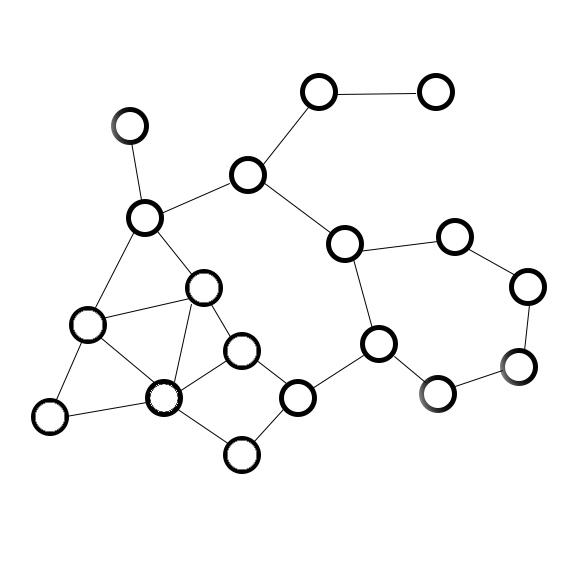
\includegraphics{images/mis1.jpg}
      	\caption{MIS : état initial}
      	\label{mis1}
   	\end{minipage} \hfill
   	\begin{minipage}[c]{.46\linewidth}
      	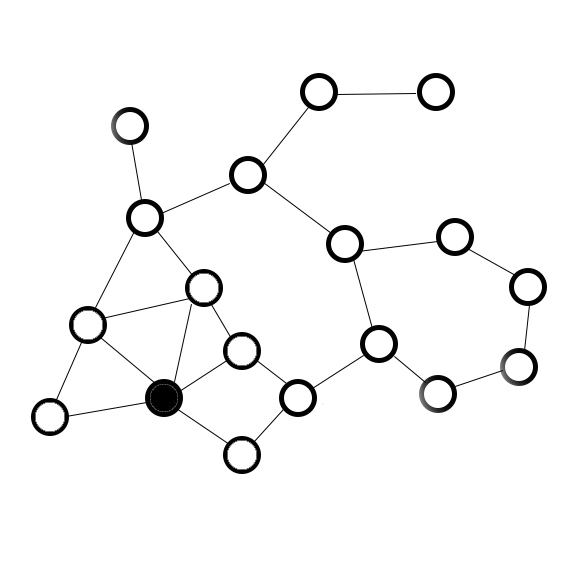
\includegraphics{images/mis2.jpg}
		\caption{MIS : leader}
		\label{mis2}
   	\end{minipage}
\end{figure}

\begin{figure}
   	\begin{minipage}[c]{.46\linewidth}
      	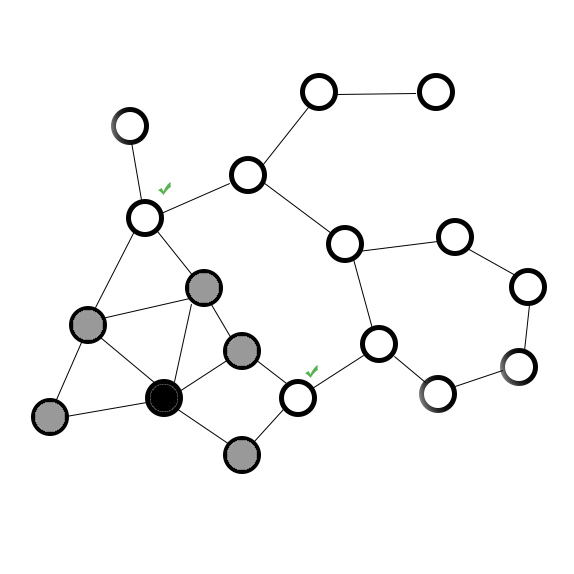
\includegraphics{images/mis3.jpg}
      	\caption{MIS : domination}
      	\label{mis3}
   	\end{minipage} \hfill
   	\begin{minipage}[c]{.46\linewidth}
      	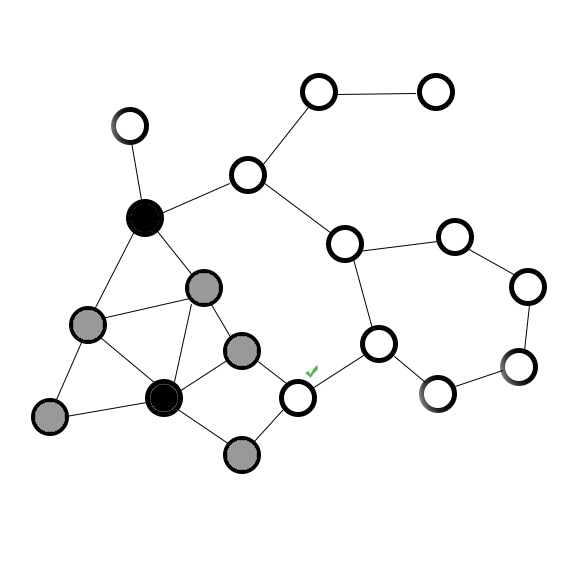
\includegraphics{images/mis4.jpg}
		\caption{MIS : élection}
		\label{mis4}
   	\end{minipage}
\end{figure}

\begin{figure}
   	\begin{minipage}[c]{.46\linewidth}
      	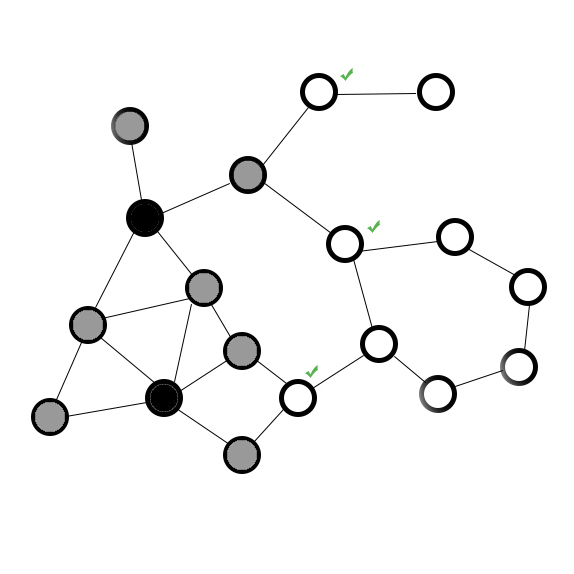
\includegraphics{images/mis5.jpg}
      	\caption{MIS : domination}
      	\label{mis5}
   	\end{minipage} \hfill
   	\begin{minipage}[c]{.46\linewidth}
      	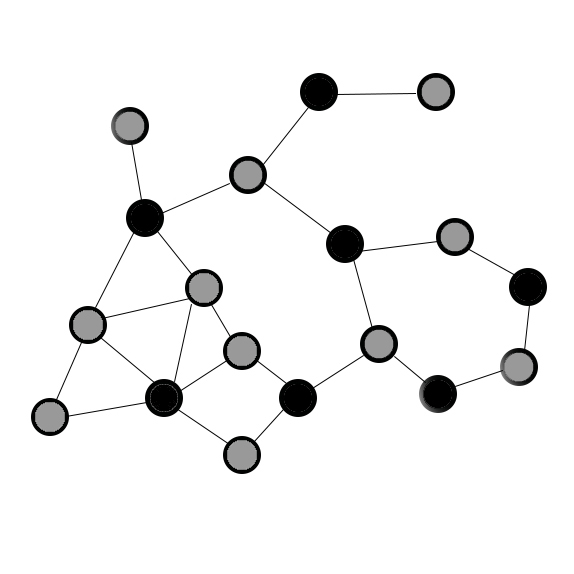
\includegraphics{images/mis6.jpg}
		\caption{MIS : état final}
		\label{mis6}
   	\end{minipage}
\end{figure}

\newpage
L'algorithme commence par choisir un tout premier nœud comme leader, en l'occurrence nous avons fait le choix de prendre le sommet de plus haut degré ce qui semble être pour nous un choix justifié puisque une plus large zone du graphe peut être couvert par ce seul point (figure \ref{mis2}. Ce nœud hôte est ainsi coloré en noir pour marqué son appartenance au MIS et tous ses voisins en gris pour indiquer leur domination par ce dernier.  (figure \ref{mis2}).
\subsection{Ensemble indépendant maximal : algorithme 2}\label{mis}

\newpage
\subsection{Construction de l'ensemble dominant connexe}
\newpage
\section{Résultats}
\subsection{Tests}

\paragraph{}
Pour tester notre algorithme nous avons eu besoin de deux choses :
\begin{itemize}
\item une fonction permettant de valider notre solution
\item un fonction permettant de générer aléatoirement des tests
\end{itemize}

\paragraph{}
La méthode \verb?isValid()? qui vérifie la validité de la solution calculée par notre algorithme est donnée par le pseudo-code suivant :
\begin{lstlisting}
isValid(ArrayList<Point> graph, ArrayList<Points> cds, int edgeTreshold) {
	valid = true;
	//build the graph structure of the cds
	ArrayList<NodeVertexDS> graphcds = graph(cds);
	
	//compute connex components
	for( v in graphcds ) {
		for( vn in v.neighbors ) {
			v.disjointsetelement.union(vn.disjointsetelement)
		}
	}
	
	compconnex = new HashSet<DisjointSetElement>();
	for( v in graphcds ) { compconnex.add(v.disjointsetelement.find()); }
	
	if(compconnex.size() > 1) { print("Error on connexity : " + compconnex.size()); valid = false) }
	
	rest = points.clone();
	rest.removeall(cds);
	
	//remove all neighbors of elements of cds from rest
	removeneighbors(rest, cds, edgeTreshold);
	
	if(rest.size() > 0) { print("Error dominating : " + rest.size()); valid = false; }
	
	return valid;
}
\end{lstlisting}

\paragraph{}
Nous avons aussi eu besoin de générer des tests. Pour cela il convient de générer des graphes géométriques de différentes tailles et avec des seuils différents (valeur maximale pour que 2 points soient considérés voisins l'un de l'autre).
Voici le pseudo code du générateur :
\begin{lstlisting}
generateGraph(width, heigth, nb, edgeTreshold) :
	result : ArrayList<Point>;
	while result.size() != nb :
		add random points in result until result.size() == nb
		compute connected components of result
		if there is multiple connected components :
			keep only the biggest connected components in points (remove the points that are in smaller components)
\end{lstlisting}

\paragraph{}
Nous avons ensuite établi plusieurs bases de test :

\begin{figure}[ht]
\begin{center}
\begin{tabular}{|*{3}{c|}}
    \hline
     Nombre de points  & Largeur $\times$ Hauteur  & Seuil \\
    \hline
    100  & 1000 $\times$ 1000 & 50 \\
    \hline
    500  & 1000 $\times$ 1000  & 50 \\
    \hline
    1000  & 1000 $\times$ 1000  & 50 \\
    \hline
    5000  & 1000 $\times$ 1000  & 50 \\
    \hline
    10000  & 1000 $\times$ 1000  & 50 \\
    \hline
\end{tabular}
\end{center}
\captionof{table}{Base de test 1}
\end{figure}

\begin{figure}[ht]
\begin{center}
\begin{tabular}{|*{3}{c|}}
    \hline
     Nombre de points  & Largeur $\times$ Hauteur  & Seuil \\
    \hline
    100  & 1000 $\times$ 1000 & 5 \\
    \hline
    500  & 500 $\times$ 500  & 25 \\
    \hline
    1000  & 1000 $\times$ 1000  & 50 \\
    \hline
    5000  & 5000 $\times$ 5000  & 250 \\
    \hline
    10000  & 10000 $\times$ 10000  & 500 \\
    \hline
\end{tabular}
\end{center}
\captionof{table}{Base de test 2}
\end{figure}

\begin{figure}[ht]
\begin{center}
\begin{tabular}{|*{3}{c|}}
    \hline
     Nombre de points  & Largeur $\times$ Hauteur  & Seuil \\
    \hline
    100  & 100 $\times$ 100 & 25 \\
    \hline
    500  & 500 $\times$ 500  & 36 \\
    \hline
    1000  & 1000 $\times$ 1000  & 50 \\
    \hline
    5000  & 5000 $\times$ 5000  & 161 \\
    \hline
    10000  & 10000 $\times$ 10000  & 300 \\
    \hline
\end{tabular}
\end{center}
\captionof{table}{Base de test 3}
\end{figure}

Base 3 : (pour cette base on souhaitait fixer edgeTreshold, cependant, un edgeTreshold de 50 pour un test de 10000 points dans un espace de 10000*10000 est trop long a générer) à la place nous avont choisi un compromis.

Une base 4 qui génère des points dans un espace beaucoup plus large que haut serait intéressante (a voir demain).

Tout ces tests seront effectués sur les deux version de l'algorithme (avec MIS1 et MIS2)

\paragraph{}
Résultats faire des graphes de taille du cds en fonction du nb de points et de temps en fonction du nombre de points pour MIS 1 et 2
4 graphes par bases (essayer de faire petit)

\begin{figure}
\begin{center}
\begin{tikzpicture}
\begin{axis}[%
  xlabel=Nombre de points,
  ylabel=Taille du CDS,
  xmin=0,
]
  \addplot[color=red,mark=x]  coordinates {
	(100, 35)
	(500, 169)
	(1000, 352)
	(5000, 377)
	(10000, 386)
};
  \addlegendentry{Base 1}
  \addplot[color=blue,mark=x]  coordinates {
	(100, 36)
	(500, 173)
	(1000, 351)
	(5000, 377)
	(10000, 384)
};
  \addlegendentry{Base 2}
  \addplot[color=green,mark=x] coordinates {
  	(100, 16)
	(500, 172)
	(1000, 352)
	(5000, 873)
	(10000, 1014)
};
  \addlegendentry{Base 3}
\end{axis}
\end{tikzpicture}
\end{center}
\captionof{figure}{Taille du CDS en fonction du nombre de points avec MIS1}
\end{figure}

BASE 1 ( 1 et 2 correspondent au MIS)
1 - 1 - 100 points - Average size : 35 points - Average time : 0.00129 s - Fails : 0
1 - 2 - 100 points - Average size : 37 points - Average time : 9.1E-4 s - Fails : 0
1 - 1 - 500 points - Average size : 169 points - Average time : 0.0046 s - Fails : 0
1 - 2 - 500 points - Average size : 174 points - Average time : 0.00425 s - Fails : 0
1 - 1 - 1000 points - Average size : 352 points - Average time : 0.01495 s - Fails : 0
1 - 2 - 1000 points - Average size : 364 points - Average time : 0.01403 s - Fails : 0
1 - 1 - 5000 points - Average size : 377 points - Average time : 0.29473 s - Fails : 0
1 - 2 - 5000 points - Average size : 394 points - Average time : 0.25969 s - Fails : 0
1 - 1 - 10000 points - Average size : 386 points - Average time : 1.16013 s - Fails : 0
1 - 2 - 10000 points - Average size : 402 points - Average time : 1.01815 s - Fails : 0

BASE 2 ( 1 et 2 correspondent au MIS)
2 - 1 - 100 points - Average size : 36 points - Average time : 2.0E-4 s - Fails : 0
2 - 2 - 100 points - Average size : 37 points - Average time : 2.4E-4 s - Fails : 0
2 - 1 - 500 points - Average size : 173 points - Average time : 0.00398 s - Fails : 0
2 - 2 - 500 points - Average size : 179 points - Average time : 0.00375 s - Fails : 0
2 - 1 - 1000 points - Average size : 351 points - Average time : 0.0149 s - Fails : 0
2 - 2 - 1000 points - Average size : 365 points - Average time : 0.01398 s - Fails : 0
2 - 1 - 5000 points - Average size : 377 points - Average time : 0.29543 s - Fails : 0
2 - 2 - 5000 points - Average size : 393 points - Average time : 0.26125 s - Fails : 0
2 - 1 - 10000 points - Average size : 384 points - Average time : 1.15217 s - Fails : 0
2 - 2 - 10000 points - Average size : 400 points - Average time : 1.01027 s - Fails : 0

BASE 3 ( 1 et 2 correspondent au MIS)
3 - 1 - 100 points - Average size : 16 points - Average time : 2.9E-4 s - Fails : 0
3 - 2 - 100 points - Average size : 18 points - Average time : 2.4E-4 s - Fails : 0
3 - 1 - 500 points - Average size : 172 points - Average time : 0.0039 s - Fails : 0
3 - 2 - 500 points - Average size : 180 points - Average time : 0.00367 s - Fails : 0
3 - 1 - 1000 points - Average size : 352 points - Average time : 0.01476 s - Fails : 0
3 - 2 - 1000 points - Average size : 365 points - Average time : 0.01395 s - Fails : 0
3 - 1 - 5000 points - Average size : 873 points - Average time : 0.32062 s - Fails : 0
3 - 2 - 5000 points - Average size : 907 points - Average time : 0.28485 s - Fails : 0
3 - 1 - 10000 points - Average size : 1014 points - Average time : 1.20708 s - Fails : 0
3 - 2 - 10000 points - Average size : 1054 points - Average time : 1.0546 s - Fails : 0
\newpage
\subsection{Discussion}
\newpage
\section{Conclusion}
%Finalement, il s'avère que l'algorithme de Toussaint est moins efficace que l'algorithme de Ritter, que ce soit en terme de temps d'exécution, d'efficacité en tant que conteneur ou même de complexité mémoire. Cependant, comme dit précédemment, c'est un algorithme qui à l'air de bien se prêter à la parallélisation. Une des raisons qui pourrait pousser à préférer l'algorithme de Toussaint à celui de Ritter serait la volonté d'obtenir un conteneur de forme rectangulaire plutôt que circulaire pour être plus fidèle à un problème posé. En effet, tout dépend de la forme globale de la répartition des points et, plus généralement, du contexte du problème considéré.

Une dernière question que l'on pourrait se poser serait celle de la validité de ces algorithmes en 3 dimensions. Fondamentalement, cela ne change pas grand chose pour l'algorithme de Ritter, l'idée générale reste la même et il suffit d'adapter les formules pour un espace de dimension 3. En revanche, cela risque d'être plus compliqué pour le rectangle qui deviendrait alors un parallélépipède. Joseph O'Rourke a proposé une solution en 1985 dont la complexité est cubique, ce qui est bien supérieur à la complexité pseudo-linéaire de la version 2D. L'idée étant que 2 des 6 faces du parallélépipède doit être coplanaire avec 2 des arêtes de l'enveloppe convexe.
\newpage
\nocite{*}
\bibliographystyle{plain}
\bibliography{bibliographie/ref}
\end{document}